\documentclass[lettersize,journal]{IEEEtran}
\usepackage{amsmath,amsfonts}
\usepackage{algorithmic}
\usepackage{array}
\usepackage[caption=false,font=normalsize,labelfont=sf,textfont=sf]{subfig}
\usepackage{textcomp}
\usepackage{stfloats}
\usepackage{url}
\usepackage{verbatim}
\usepackage{fancyvrb,fvextra}
\usepackage{graphicx}
\usepackage{xcolor}
\def\BibTeX{{\rm B\kern-.05em{\sc i\kern-.025em b}\kern-.08em
    T\kern-.1667em\lower.7ex\hbox{E}\kern-.125emX}}
\usepackage{balance}
\usepackage[square, numbers]{natbib}
\begin{document}
\title{CPTR380 RISC-V RV32I FPGA Implementation}
\author{Jaron Brown \& Ethan Jansen
\thanks{Manuscript created March, 2024.}}

\maketitle

\begin{abstract}
\color{red}{TBD}
\end{abstract}

\begin{IEEEkeywords}
ISA, RISC, RISC-V, RV32I FPGA, VHDL.
\end{IEEEkeywords}


\section{Introduction}
\IEEEPARstart{S}{ince} designing a custom accumulator-based CPU last quarter for the Intro to Digital Design class, 
both of the authors developed an interest in implementing a more commonly supported instruction set architecture (ISA). 
When presented with the opportunity to pursue a project related to computer architecture in their Computer Architecture class, 
both authors jumped at the opportunity to implement another CPU design.
They initially considered implementing the MIPS (Microprocessor without Interlocked Pipelined Stages) ISA, which was being studied in class, but, 
after conducting more research, decided on implementing one of the RISC-V standard ISAs, RV32I.
This keeps with the RISC (Reduced Instruction Set Computer) design, and takes advantage of the abundant documentation for the RISC-V ISAs, RV32I's relative simplicity, the high commercial interest in these ISA specifications,
and in the interest in supporting open-source projects.

One of the dominant reasons many companies are developing RISC-V implementations is its open-source nature \cite{riscvhistory}. 
The dominant ISAs (x86, ARM, MIPS, etc.) all have steep licensing fees.
The RISC-V ISAs, in comparison, are completely free. 
Having a completely open-source ISA just makes sense--it lowers the barrier to entry for designing hardware to implement standard 
ISAs and allows for more innovation in the realm of CPU design.  

\section{A Brief Introduction to RISC-V}
The original design of RISC-V was begun in 2010 at the University of California, Berkeley. 
It was designed not only as an academic learning aid but also as a set of ISAs that could have commercial viability \cite{riscvhistory}. 
As its name suggests, RISC-V is a RISC architecture. 
This means, in comparision to CISC (Complex Instruction Set Computer) ISAs, RISC ISAs have simple instructions. 
This means more individual instructions will be required to complete a given task compared to CISC ISAs but also allows the 
hardware implementation to be much simpler than that for CISC ISAs.
In fact, even implementations of x86-64, the most widely adopted CISC ISA, breaks its CISC instructions into "microinstructions" which are easier to implement in hardware, similar to RISC ISAs \cite{cisctorisc}.

RISC-V is not actually \textit{an} ISA but rather a collection of ISAs, 
ranging from 32-bit to 128-bit standards and supporting various levels of complexity by way of extensions to the base ISAs \cite{riscvunprovisioned}. 
Some official extensions include the M extension which adds multiplication and division support, 
the A extension which adds support for atomic instructions, and the F and D extensions which add support for single- and double-precision floating numbers, 
respectively \cite{riscvunprovisioned}. Developers are encouraged to design their own compatible extensions to customize the base RISC-V ISA to their specific application.

In this project, revision 2.1 of the RV32I unprivileged ISA will be implemented in VHDL and tested on a Xilinx Artix 7 FPGA (Field-Programmable Gate Array). 
RV32I is the RISC-V 32-bit base integer ISA and implements the core functionality of the RISC-V architecture family \cite{riscvunprovisioned}.
Using this, the implemented microcontroller should easily support C code cross-compilation via clang after future I/O library support.
This will help test/debug the microcontroller during implementation.
Even more notable, however, is this will greatly improve the accessibility of this project as a useful processor.

\subsection{Stretch Goals}
The following goals would all improve the design, however are not necessary to meet a basic RV32I implementation.
Because of time constraints these are items are not actively being pursued.
\begin{itemize}
    \item I/O: I/O support is not part of RV32I. Because of this, an extension, or a co-processor, would be needed for proper implementation.
        For these reasons, proper I/O implementation is a stretch goal. However, because basic I/O support is required for testing/debugging, it will be unofficially
        implemented.
    \item Pipelining: Although RV32I supports pipelining, this project's implemetation will not implement this feature due to projected time constraints.
        Pipelining is not necessary to meet ISA requirements, and the lack of pipelining will only increase the clock cycles per instruction (CPI) but will greatly
        simplify the control logic and data path unit (DPU).
    \item Multiplication \& Division: These are technically part of the M extension \cite{riscvunprovisioned} and thus are not high priorities.
        However, because \verb|IEEE.numeric_std| (the VHDL library) has built in support for multiplication and division this would not be difficult to add to
        the existing arithmetic logic unit (ALU). The ALU would simply require another bit of control.
    \item Standard C Code Compilation Support: Basic C support is planned for this project, however exensive support is currently not guaranteed.
\end{itemize}
The authors intend to continue supporting this project by refining the design and implemented the discussed stretch goals.
 
\section{Understanding RV32I}
The RV32I ISA defines four main instruction types, with an additional two instruction types which are subsets of the main instruction types \cite{riscvunprovisioned}.
They are as follows:
\begin{itemize}
  \item R-type: Supports integer register-register arithmetic operations
  \item I-type: Supports integer register-immediate arithmetic operations
  \item S-type: Supports store instructions
  \item B-type (SB-type): Supports branch instructions
  \item U-type: Supports load upper immediate (\verb|LUI|) and add upper immediate to \verb|pc| (\verb|AUIPC|) instructions
  \item J-type (UJ-type): Supports jump and link (\verb|JAL|) instructions
\end{itemize}
While there are various types, they are structured in a way as to maintain as much consistency as possible.
For instance, the opcode, destination register, and source registers are always located in the same part of the binary-coded instruction.
Futhermore, the immediates are positioned as to keep the sign-extension bit in bit 31 of the instruction, and to keep the other bits of the immediates as consistent as possible.
This sometimes requires unscrambling the B-type and J-type immediates--as indicated by the blocks in Figure 5--however eliminates unnecessary fan-out \cite{riscvunprovisioned} and simplifies the overall implementation.

The RV32I ISA also specifies 40 instructions.
They are as follows:
\begin{itemize}
  \item Register-Immediate:
  \begin{itemize}
    \item I-type: \verb|ADDI, SLTI[U], ANDI, ORI, XORI|
    \item Special Shift I-type: \verb|SLLI, SRLI, SRAI|
    \item U-type: \verb|LUI, AUIPC|
  \end{itemize}
  \item Register-Register:
  \begin{itemize}
    \item R-type: \verb|ADD, SLT[U], AND, OR, XOR, SLL,|
     \verb|SRL, SUB, SRA|
  \end{itemize}
  \item Unconditional Jumps:
  \begin{itemize}
    \item J-type: \verb|JAL|
    \item I-type: \verb|JALR|
  \end{itemize}
  \item Conditional Branches:
  \begin{itemize}
    \item B-type: \verb|BEQ, BNE, BLT[U], BGE[U]|
  \end{itemize}
  \item Load \& Store:
  \begin{itemize}
    \item I-type: \verb|LW, LH[U], LB[U]|
    \item S-type: \verb|SW, SH, SB|
  \end{itemize}
  \item Memory Ordering:
  \begin{itemize}
    \item \verb|FENCE|
  \end{itemize}
  \item Environment Call \& Breakpoints:
  \begin{itemize}
    \item I-type: \verb|ECALL, EBREAK|
  \end{itemize}
\end{itemize}

Most of the Register-Immediate and Register-Register are the usual arithmetic operations with are performed primarily by the ALU.
There are a few exceptions, however, \verb|SLTI| and \verb|SLTIU| perform the same operation--setting the destiation register equal to one if the first source is less than the second--the difference is that one performs signed comparison while the other performs unsigned comparison.
This requires supporting signed and unsigned comparison flag outputs from the ALU.
The other exceptions are the U-type \verb|LUI| and \verb|AUIPC|.
The \verb|LUI| instruction loads a 20-bit immediate into the upper bits of the destination register and thus does not require the ALU, only some zero-padding to 32 bits.
The \verb|AUIPC| instruction allows creating program counter (PC) relative addresses and thus requires a byte-addressed PC input into the ALU.
None of these instructions raise exceptions.

The unconditional jump instructions are as one would expect, however the \verb|JAL| instruction notably uses a J-type immediate in order to encode more bits, thus requiring some unscrambling.
Both of these instructions allow for modifying to PC in order to jump. While \verb|JAL| uses a PC relative offset, \verb|JALR| uses an offset relative to a base register.
These instructions can also raise an \verb|Instruction-address-misaligned| exception if the target address is not aligned to a word (4 byte) boundary.
This indicates the need for some basic exception handling.
A proposed solution for this preliminary design is to store the exceptions as flags in some "exception-flags" control register.

The conditional branches are similar to the unconditional jumps, but this time implemented as B-type instructions in order to perform register comparison.
The ALU will handle this comparison via signed and unsigned subtraction and then output the necessary flags.
If the appropriate ALU flags are raised the control will signal for the PC to take on a value corresponding to the B-type immediate (which requires unscrambling) offset.
These instructions may also raise an \verb|Instruction-address-misaligned| exception.

The load and store instructions are encoded using I- and S-type instructions, respectively.
The difference in instruction types come from store needing two source registers--one for a base adress and one to store into--while the load instructions only require one register--for the base address.
The instructions also support loading/storing bytes and half-words.
While loading bytes (\verb|LB[U]|) and half-words (\verb|LH[U]|) is relatively straightforward--the upper bits can simply be masked off or signed extended as necessary--storing bytes (\verb|SB|) and half-words (\verb|SH|) is more complicated as the upper bits are not replaced on a store.
Futhermore, when performing byte and half-word operations the addresses are aligned according to the byte or half-word, rather than keeping the address word-aligned.
This requires some extra control and alignment checks as well as some built-in byte/half-word support for the Data Memory and I/O (as it will be treated as data memory) as shown in Figure 2.
These instructions will also raise \verb|Address-misaligned| or \verb|Access-fault| exceptions if the address is not naturally aligned or if out of range.

The additional memory ordering, environment call, and breakpoint instructions are less relevant to this preliminary design.
There purpose is to support reading/writing to memory from different coprocessors, as well as to support some priveleged operating system and debugger functions.
Because this does not yet apply to this project, the predecessor/successor I/O and read/write bits of the \verb|FENCE| instruction are simply saved to a control register as shown in figure 5 \cite{riscvunprovisioned}.
Futhermore, the \verb|ECALL| instruction is treated as a \verb|NOP| while the \verb|EBREAK| instruction is treated as a \verb|HALT| for some possible future hardware-controlled halt and single-step (where CPU operation automatically halts between instructions or between pipeline stages) support.

The deep understanding of these instructions is pivotal to this project and drives the data path unit (DPU) and controller implementations.

\section{Implementation}
\subsection{Overview}
This project's implementation of non-pipelined RV32I consists of a few core components:
\begin{itemize}
    \item instruction \& data memory (separated)
    \item a register file
    \item an ALU
    \item various other DPU components related to sign-extension, incrementing the program counter, branching, and routing signals
    \item a control module
\end{itemize}
Unlike the authors' previous CPU designs which used an accumulator-based design, 
this implementation uses a register file with 32 32-bit wide registers.
Besides the different ISA support (the original accumulator-based CPU used a custom ISA),
the switch to using a bank of registers is the most significant hardware design change between the two implementations.
This change, however, is in keeping with the RV32I standard and allows for more flexibility when programming the CPU.

\subsection{Program Counter}
\begin{figure}[!h]
  \label{fig:pc}
  \centering
  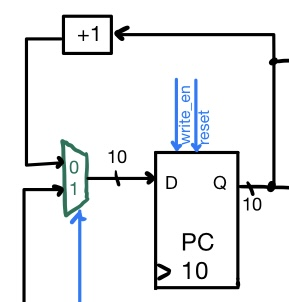
\includegraphics[width=5cm]{PC.jpg}
  \caption{Program Counter with Branch \& Jump Support}
\end{figure}

\subsection{Instruction Memory,  Data Memory, and I/O}
\begin{figure}[!h]
    \label{fig:memory}
    \centering
    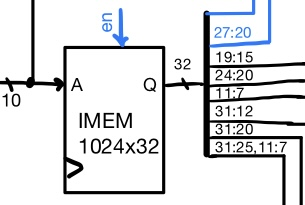
\includegraphics[width=5cm]{IMEM.jpg}
    \rule{7cm}{0.8pt}
    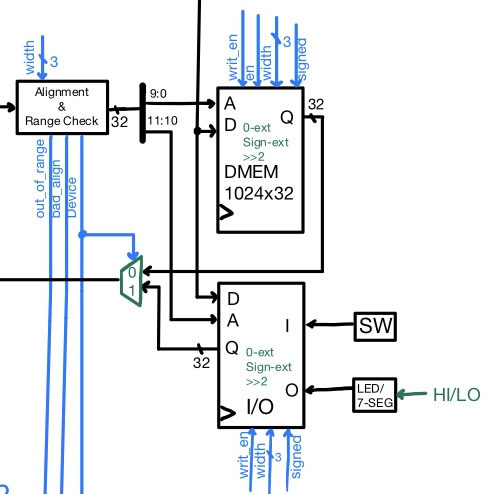
\includegraphics[width=5cm]{DMEM-IO.jpg}
    \caption{Instruction Memory (top). Data Memory with I/O Support (bottom).}
\end{figure}
Each memory (instruction and data) block was implemented in VHDL using AMD's write-first memory example using an array of \verb|std_logic_vector|s \cite{amdblockram}.
This allows for quick implementation; furthermore, it ensures that the memory blocks will be mapped to a physical FPGA memory block for improved performance
--the clock will not have to be further delayed as it may have been otherwise.

One change from AMD's example that needed to be made was support writing bytes and half-words for data memory.
This is to support the \verb|sb| and \verb|sh| instructions as they do not overwrite the upper bits.
Without the additional support baked into the data memory,
an additional register would need to be added to temporarily hold the upper bits so that they do not get overwritten--this would require additional clock cycles to implement.

The instruction memory has been implemented and holds a maximum of 1024 32-bit instructions.
Because the implementation does not support all of RV32I's 32-bit ($2^{32}$) addresses, the lower ten bits are masked and are used as the instruction memory address.
The current implementation of instruction memory is untested.
Currently, data memory is not implemented due to time constraints.
When implemented, data memory will hold 1024 32-bit wide values and will support read and write.
As per RV32I specification, data memory will support storing/loading word, halfwords, and bytes.
\color{red}{Incomplete..}\color{black}\\
\subsection{Register File}
\begin{figure}[!h]
    \label{fig:regblock}
    \centering
    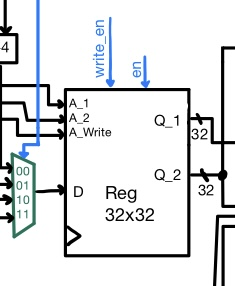
\includegraphics[width=5cm]{REG.jpg}
    \caption{32-bit Register File}
\end{figure}
The implementation of the register block fully supports the RV32I specification.
Register \verb|x0| is writable but, when read, always returns a vector of zeros and the other generic registers (\verb|x1|-\verb|x31|) function according to the RV32I specification.
The control signals to the register block are \verb|write-enable| and \verb|enable|.
These control signals are important as they lock the register block so nothing changes (\verb|enable|) or, when \verb|enable| is held high, allow writes to the registers (\verb|write-enable|).
Locking the register block so nothing changes (using \verb|write-enable|) is important in this non-pipelined implementation where the values of different components need to remain
 stable after being updated by an instruction for the remaining clock cycles required to complete that instruction.
The register block is implemented using a write-first memory block which is an array of \verb|std_logic_vector|s, similar to how the instruction memory is implemented.
Custom logic is implemented to allow for two registers to be read at once.

This implementation has been tested using the VHDL testbenches built into ISE.
Tests include reading and writing to registers, reading and writing to register \verb|x0|, and writing to and reading from the same register.


\subsection{ALU}
\begin{figure}[!h]
    \label{fig:alublock}
    \centering
    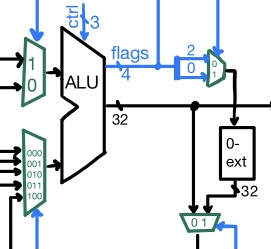
\includegraphics[width=5cm]{ALU.jpg}
    \caption{ALU with Conrol Flag Output}
\end{figure}
The arithmetic logic unit (ALU) is a fully combinational block which will perform the desired arithmetic operation based on the input control lines.
Shown in Table I are the main operations the ALU is required to support. Because there are various instructions associated with the same
arithmetic operation (such as needing to determine the address used for load and store using ADD) the control line into the ALU is only 3-bits wide in order to support
the eight different arithmetic operations, but the actual control signal is determined from a separate "ALU Control" block rather than directly from the instruction.
In addition to arithmetic operations, the ALU performs comparisons between the two inputs, which are used for branch conditions and for the SLTI and SLTIU instructions.
These comparisons are made visible through four flags: unsigned less-than and greater-than and signed less-than and greater-than.
With these four flag outputs any of the signed and unsigned branch conditions can be supported:
\begin{itemize}
    \item BEQ: equals
    \item BNE: not equals
    \item BLT \& BLTU: less-than
    \item BGE \& BGEU: greater-than
\end{itemize}
Furthermore, SLT, SLTU, SLTI \& SLTIU (set less-than) instructions can be supported by selecting between the signed and unsigned less-than flags (using a mux), zero-extending the one-bit value, and selecting it as an output (via another mux) instead of the ALU's arithmetic result.
The set less-than instructions set the least-significant bit (LSB) of an otherwise zero 32-bit vector to 1 or 0 depending on if the first input is less-than/greater-than the second input, respectively.

The ALU has been tested using the VHDL testbenches built into ISE.
All the core arithmetic functions have been tested.
Additionally, the four comparison flags have been tested in all their combinations.
One might expect full coverage testing of the flags to require $2^{4}$ tests but, since the flags are not independant, the total number of required tests is reduced to five.

This ALU Control block takes in \verb|opcode, funct3|, and \verb|funct7| from the encoded instruction and translates this into the necessary 3-bit ALU control signal.
Separating this block also allows more easily decoding the necessary information from the six different \cite{riscvunprovisioned} instruction types.
\begin{table}
    \label{table:ALUOps}
    \centering
    \begin{tabular}{|p{2.7cm}|p{4cm}|}
        \hline
        Operation & Instructions \\
        \hline\hline
        ADD & ADD(I),\newline Load \& Store (various),\newline JALR, AUIPC\\
        SUB & SUB, SLT (various),\newline Branch (various)\\
        XOR & XOR(I)\\
        OR & OR(I)\\
        AND & AND(I)\\
        Left Shift & SLL(I)\\
        Right Shift & SRL(I)\\
        Right Shift (Arith.) & SRA(I)\\
        \hline
    \end{tabular}
    % there seems to be a caption spacing issue. probably related to IEEE, may just end up using figure
    \vspace{4pt}
    \caption{RV32I Base Arithmetic Operations Matched to the Instructions}
\end{table}


\subsection{DPU Miscellaneous}
\begin{figure}[!h]
  \label{fig:dpumisc}
  \centering
  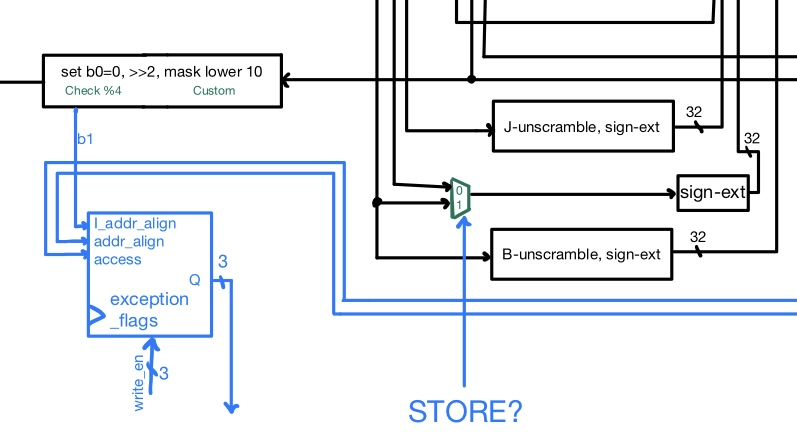
\includegraphics[width=5cm]{Misc1.jpg}
  \rule{7cm}{0.8pt}
  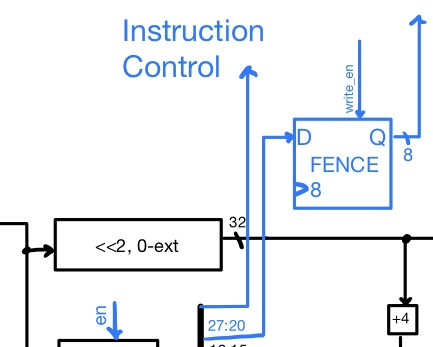
\includegraphics[width=5cm]{Misc2.jpg}
  \caption{Stuff}
\end{figure}
\color{red}{TBD}\color{black}

\subsection{Control}
\color{red}{Incomplete...}\color{black}\\
The control is primarily separate from the DPU (apart from a few components such as the ALU control).
This nicely separates the control from the rest of the CPU processing and makes a nice division in the design.
We were able to do this by not considering pipelining, thus removing any forwarding registers and branch prediction modules from being interweaved into the DPU.

However, because there is no pipelining, the controller needs to be aware of how long each instruction takes to execute.
This is mostly separated into the six different instruction types--where each instruciton within an instruction type takes the same number of clock cycles to execute.
For the current implementations, the instruction length is hardcoded into the controller. For instance, the controller will wait four clock cycles for an ADD to execute
before continuing to the next instruction.

The controller also has support of pausing and single-stepping.
This greatly improves the debugging of the device.
This is useful not only during hardware design of the CPU but also when writing software to run on the CPU.
Currently, however, there is no proper I/O support, so there are dedicated buttons on the FPGA board to control the single-stepping.
Thus, single-stepping can not be controlled via a software debugger.
This is planned for future work.

\section{Testing \& Design Review}
To verify this project's RISC-V implementation is valid, a few methods can be used. First of all, the individual modules must be tested in isolation.
This can be done one of two ways: implementing testbenches in either VHDL or Python using either simulation testbenches or by creating testing wrappers which provide inputs to the modules and display the outputs on either the LEDs, seven-segment display, or digital pins on the FPGA board.
Two compelling options for implementing testbenches are utelizing the VHDL testbench tools built into ISE or using cocotb.
Testbenches are definitely the prefered way to test since they cut out some of the opportunity for error that comes from setting switches and reading LEDs.
Additionally, they allow for automated pass/fail tests and provide timing diagrams, which simplify debugging significantly compared to testing on hardware.
The VHDL testbench tools built into Xilinx ISE are relatively simple to use and auto generate the component imports.
Additionally, the ISE testbench tools provide timing diagrams for the tests, which was found useful for this project.
cocotb is a testbench suite which allows users to define testbenches in Python.
It has many compelling features but the time required to setup and learn the tool was prohibitive.
Since both authors are already familiar with Xilinx ISE for its synthesis and FPGA configuration tools, they opted to use the ISE testbench tools.
The ISE VHDL testbenches were fairly simple to learn and using them for component testing saved the authors a significant amount of time.

\section{Conclusion}
\color{red}{TBD}\color{black}

{\appendices
\section*{Complete Data Path Unit Block Diagram}
\begin{figure}[!h]
  \label{fig:dpu}
  \centering
  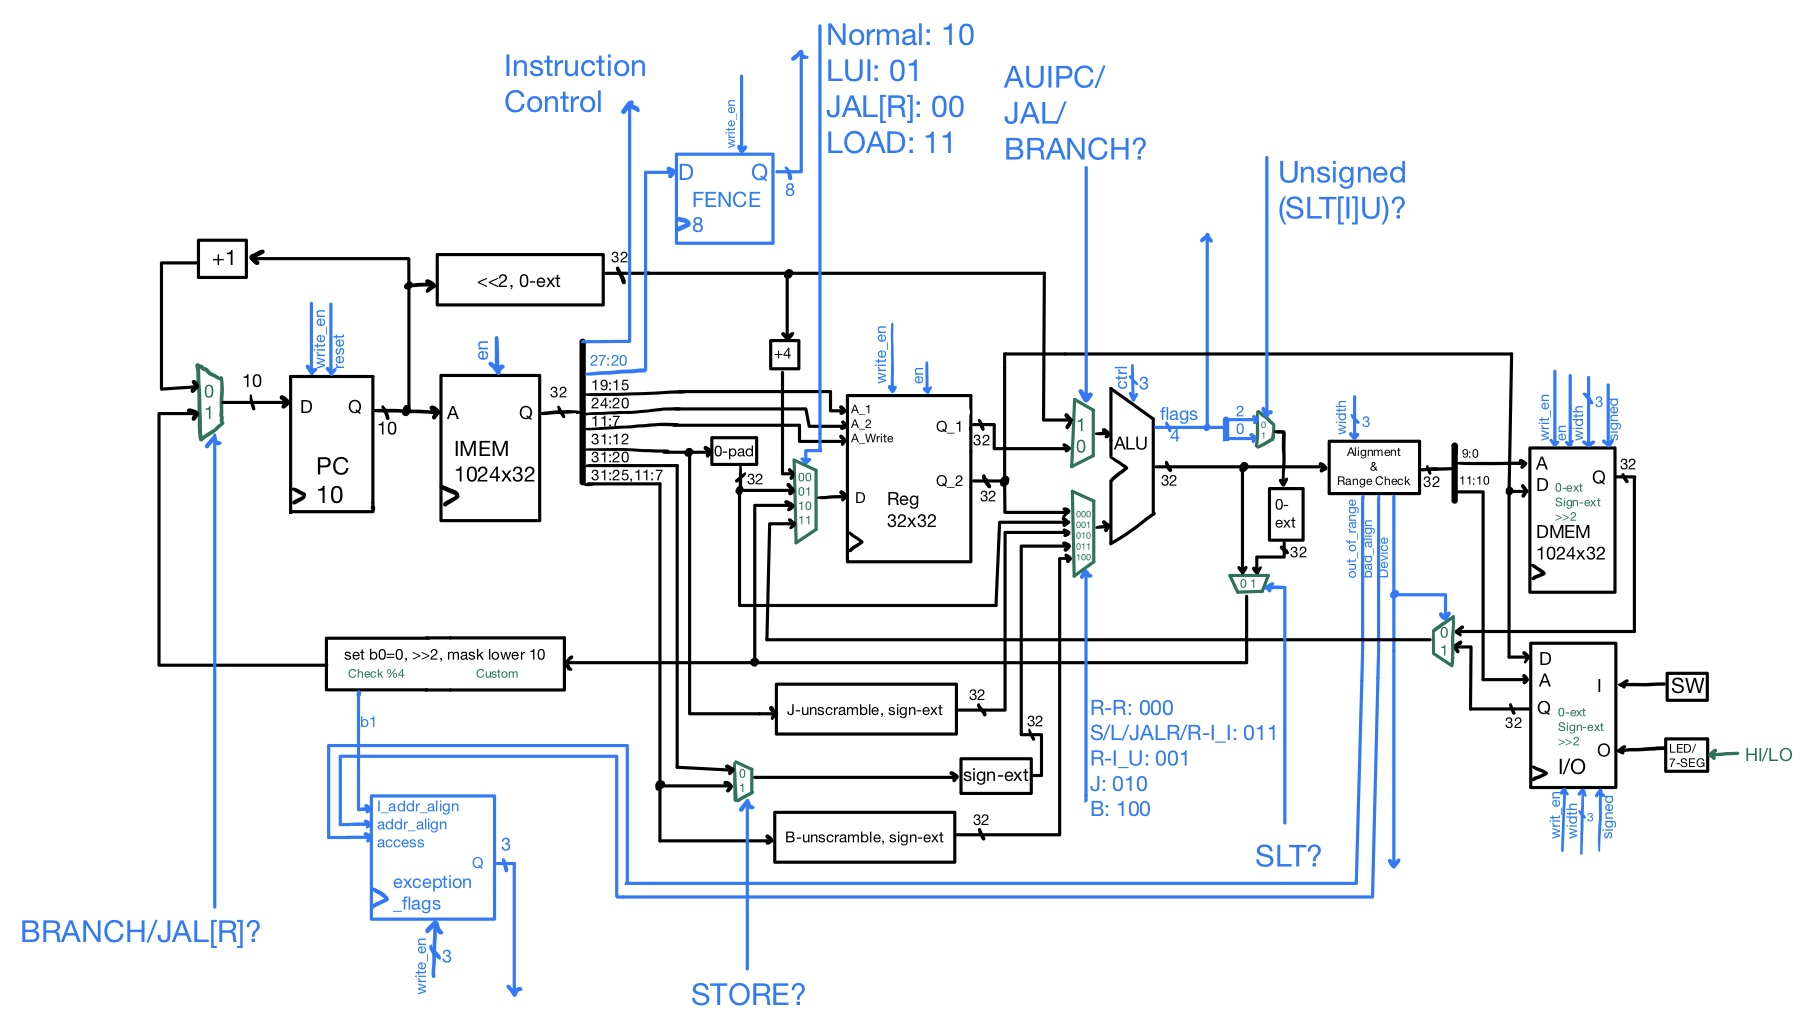
\includegraphics[width=16cm, angle=270]{DPU.jpg}
  \caption{Data Path Unity with Control Signals (blue)}
\end{figure}

\section*{VHDL Implementations}
Sample:
\color{red}{TBD due to current overfull issues...}\color{black}\\
\subsection{Program Counter}
\begin{Verbatim}[breaklines]
  library IEEE;
  use IEEE.std_logic_1164.all;
  
  entity program_counter is
    port
    (
      clk   : in std_logic; --! Clock
      reset : in std_logic; --! Reset to 0
      en    : in std_logic; --! Enable
      D     : in std_logic_vector(9 downto 0); --! New pc
      Q     : out std_logic_vector(9 downto 0) --! Current pc
    );
  end program_counter;
  
  architecture pc of program_counter is
  begin
    process (clk)
    begin
      if rising_edge(clk) then
        if reset = '1' then
          Q <= "0000000000";
        elsif en = '1' then
          Q <= D; --! When reset != 0 and en = 1
        else
          Q <= Q; --! When reset != 0 and en = 0
        end if;
      end if;
    end process;
  
  end pc;
\end{Verbatim}
\subsection{Instruction Memory}
\begin{Verbatim}[breaklines]
  library IEEE;
  use IEEE.std_logic_1164.all;
  use IEEE.numeric_std.all;
  use IEEE.std_logic_textio.all;
  use std.textio.all;
  
  entity rom_with_init is
    port
    (
      clk  : in std_logic; --! Clock
      en   : in std_logic; --! Enable
      addr : in std_logic_vector(9 downto 0); --! Address
      d    : out std_logic_vector(31 downto 0) --! Data Out
    );
  end rom_with_init;
  
  architecture rom of rom_with_init is
    type rom_type is array(0 to 1023) of std_logic_vector(31 downto 0);
  
    impure function initRomFromFile(romFileName : in string) return rom_type is
      file romFile                                : text is in romFileName;
      variable romFileLine                        : line;
      variable rom                                : rom_type;
    begin
      for i in rom_type'range loop
        readline(romFile, romFileLine);
        read(romFileLine, rom(i));
      end loop;
      return rom;
    end function;
  
    signal rom : rom_type := initRomFromFile("rom.data");
  begin
    process (clk)
    begin
      if rising_edge(clk) then
        if en = '1' then
          d <= rom(to_integer(
            unsigned(addr)));
        end if;
      end if;
    end process;
  end rom;
\end{Verbatim}
\subsection{ALU}
\begin{Verbatim}[breaklines]
  library IEEE;
  use IEEE.STD_LOGIC_1164.all;
  use IEEE.NUMERIC_STD.all;
  
  entity arithmetic_logic_unit is
    port
    (
      ctrl               : in std_logic_vector(2 downto 0); --! From control module
      data1_in, data2_in : in std_logic_vector(31 downto 0); --! Assuming immediate sign extensions happen outside of alu
      data_out           : out std_logic_vector(31 downto 0);
      flags              : out std_logic_vector(3 downto 0)
    );
  end arithmetic_logic_unit;
  
  architecture alu of arithmetic_logic_unit is
    constant sel_add                         : std_logic_vector(2 downto 0) := "000";
    constant sel_sll                         : std_logic_vector(2 downto 0) := "001";
    constant sel_sub                         : std_logic_vector(2 downto 0) := "010";
    constant sel_sra                         : std_logic_vector(2 downto 0) := "011";
    constant sel_xor                         : std_logic_vector(2 downto 0) := "100";
    constant sel_srl                         : std_logic_vector(2 downto 0) := "101";
    constant sel_or                          : std_logic_vector(2 downto 0) := "110";
    constant sel_and                         : std_logic_vector(2 downto 0) := "111";
    signal nonzero_s, nonzero_u              : std_logic;
    signal shift                             : std_logic_vector(4 downto 0);
    signal sig_sra                           : std_logic_vector(31 downto 0);
    signal sig_xor, sig_srl, sig_or, sig_and : std_logic_vector(31 downto 0);
    signal sig_sll                           : unsigned(31 downto 0);
    signal sig_add, sig_sub                  : signed(31 downto 0);
    signal unsigned_ext_1, unsigned_ext_2    : std_logic_vector(32 downto 0);
    signal sig_unsigned_comp                 : signed(32 downto 0);
  
  begin
    -- signals all calculated to be muxed via ctrl
  
    -- logic
    shift   <= data2_in(4 downto 0);
    sig_add <= signed(data1_in) + signed(data2_in);
    sig_sll <= shift_left(unsigned(data1_in), to_integer(unsigned(shift)));
    sig_sub <= signed(data1_in) - signed(data2_in);
    sig_sra <= std_logic_vector(shift_right(
      signed(data1_in), to_integer(unsigned(shift))));
    sig_xor <= data1_in xor data2_in;
    sig_srl <= std_logic_vector(shift_right(
      unsigned(data1_in), to_integer(unsigned(shift))));
    sig_or  <= data1_in or data2_in;
    sig_and <= data1_in and data2_in;
  
    nonzero_s <= '0' when sig_sub = X"00000000" else
      '1'; --! Check difference is non-zero
    flags(3)          <= (not sig_sub(31)) and nonzero_s; --! Positive and non-zero
    flags(2)          <= sig_sub(31); --! Sign bit of signed subtraction operation
    unsigned_ext_1    <= '0' & data1_in; --! Effectively create positive signed value from unsigned
    unsigned_ext_2    <= '0' & data2_in; --! Effectively create positive signed value from unsigned
    sig_unsigned_comp <= signed(unsigned_ext_1) - signed(unsigned_ext_2);
    nonzero_u         <= '0' when sig_unsigned_comp = "000000000000000000000000000000000" else
      '1'; --! Check difference is non-zero
    flags(1) <= (not sig_unsigned_comp(32)) and nonzero_u;
    flags(0) <= sig_unsigned_comp(32);
    -- signal select mux
    with ctrl select
      data_out <=
      std_logic_vector(sig_add) when sel_add,
      std_logic_vector(sig_sll) when sel_sll,
      std_logic_vector(sig_sub) when sel_sub,
      sig_sra when sel_sra,
      sig_xor when sel_xor,
      sig_srl when sel_srl,
      sig_or when sel_or,
      sig_and when others;
  end alu;
\end{Verbatim}
\subsection{Register File}
\begin{Verbatim}[breaklines]
  library IEEE;
  use IEEE.std_logic_1164.ALL;
  use IEEE.NUMERIC_STD.ALL;
  
  entity register_block is
      port
      (
        clk               : in std_logic; --! Master clock
        we                : in std_logic; --! Write enable
        en                : in std_logic; --! Keeps Q_1 and Q_2 from changing
        A_1, A_2, A_Write : in std_logic_vector(4 downto 0); --! Address inputs
        D                 : in std_logic_vector(31 downto 0); --! Data in
        Q_1, Q_2          : out std_logic_vector(31 downto 0) --! Data out
      );
  end register_block;
  
  architecture reg_blk of register_block is
    type reg_type is array (31 downto 0) of std_logic_vector(31 downto 0);
    signal REG : reg_type := (others=>(others=>'0'));
  
    
  begin
    process(clk)
    begin
      if rising_edge(clk) then
        if en = '1' then
          if we = '1' and A_Write /= "00000" then
            REG(to_integer(unsigned(A_Write))) <= D;
            if (A_Write = A_1) and (A_Write = A_2) then
              Q_1 <= D;
              Q_2 <= D;
            elsif (A_Write = A_1) then
              Q_1 <= D;
              Q_2 <= REG(to_integer(unsigned(A_2)));
            elsif (A_Write = A_2) then
              Q_2 <= D;
              Q_1 <= REG(to_integer(unsigned(A_1)));
            else
              Q_1 <= REG(to_integer(unsigned(A_1)));
              Q_2 <= REG(to_integer(unsigned(A_2)));
            end if;
          else
            Q_1 <= REG(to_integer(unsigned(A_1)));
                 Q_2 <= REG(to_integer(unsigned(A_2)));
          end if;
                  
        end if;
      end if;
    end process;
  end reg_blk;
\end{Verbatim}
}

\nocite{*}
\bibliographystyle{IEEEtran}\bibliography{IEEEabrv,bibliography}

\end{document}


